\chapter{The HPS Detector}

The HPS detector is a spectrometer with a silicon vertex tracker for momentum measurement and a electromagnetic calorimeter for energy measurement and trigger.
The detector is installed in the middle dipole of a three-magnet chicane, with the field extending from the target foil to the end of the tracker.

\begin{figure}[ht]
    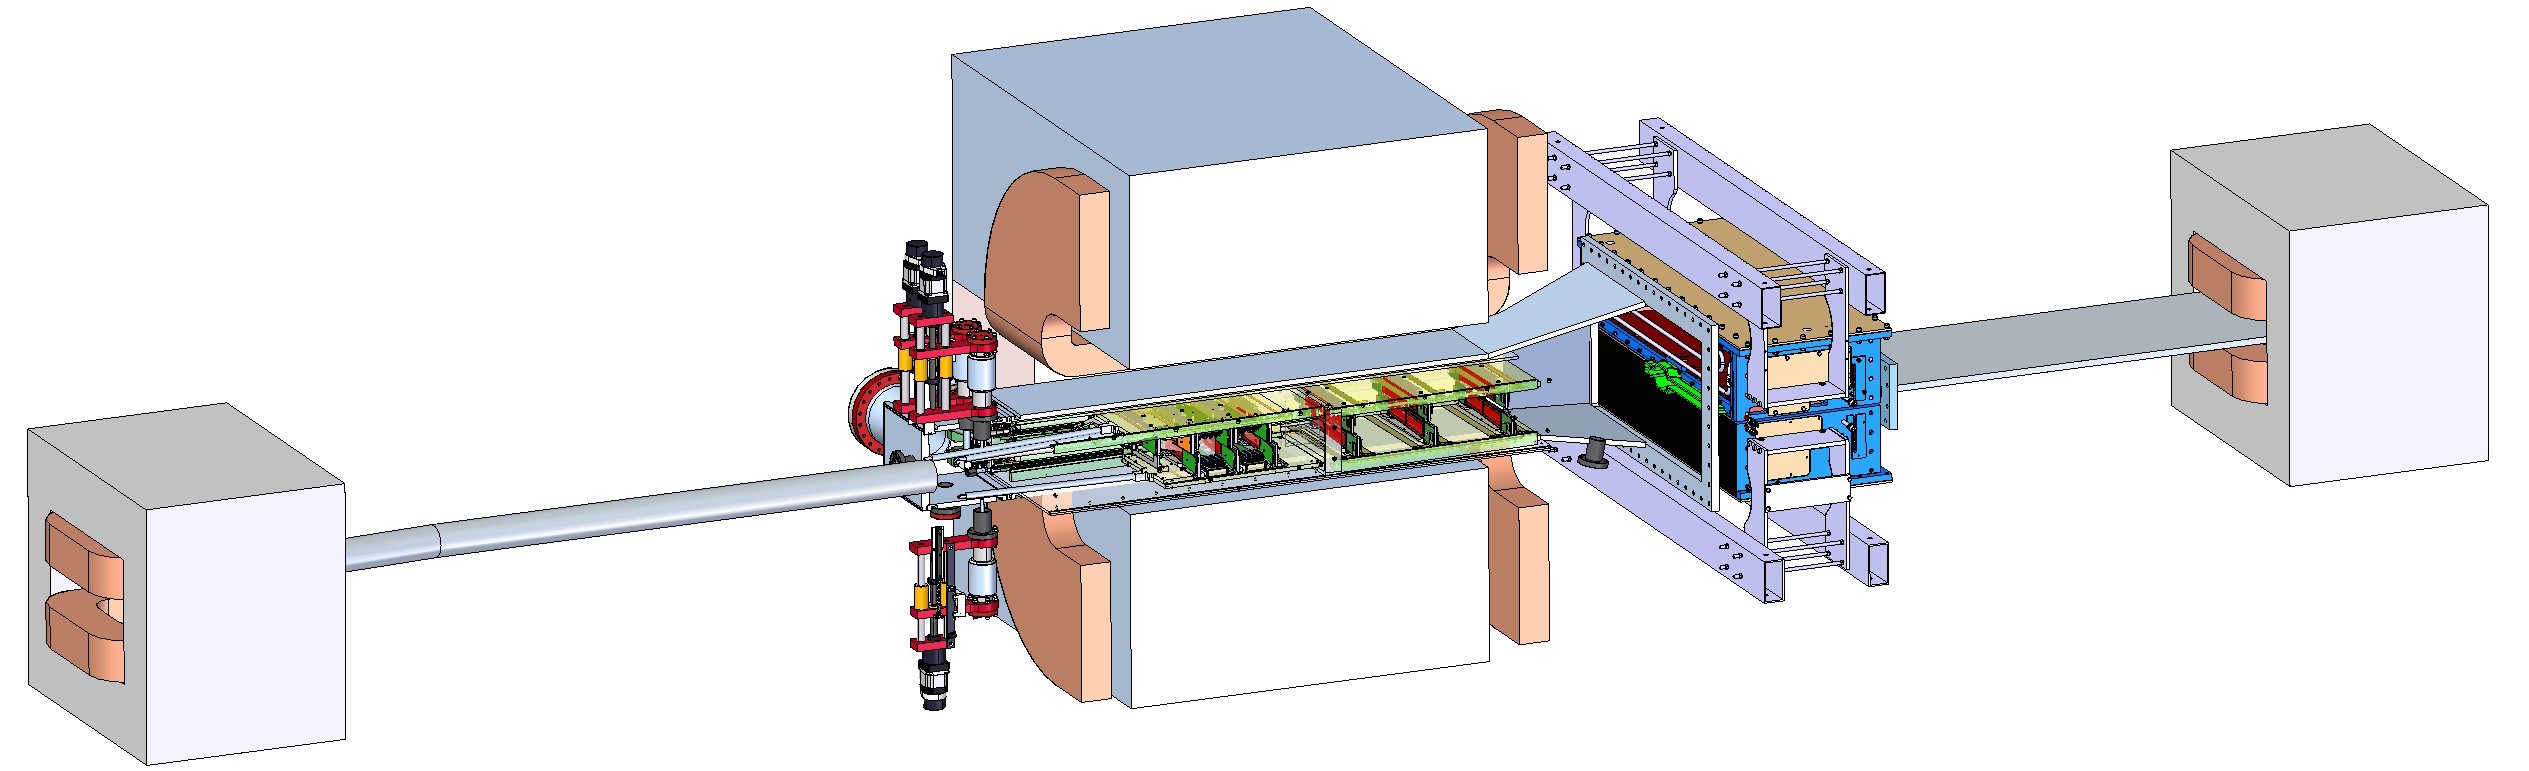
\includegraphics[width=\textwidth]{detector/figs/HPS-pic}
    \caption{View of the HPS setup.}
    \label{figure:svt_layout}
\end{figure}

\begin{figure}[ht]
    \begin{center}
    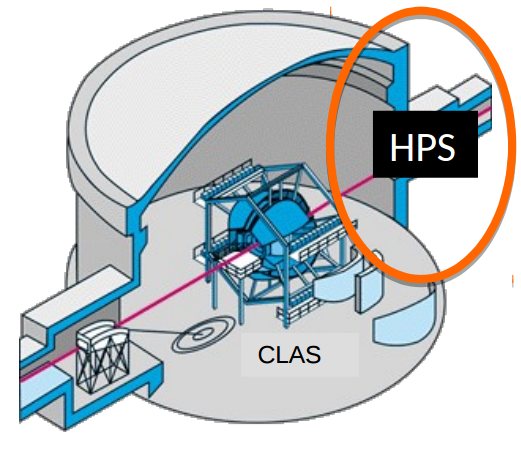
\includegraphics[width=0.5\textwidth]{detector/figs/hallb}
\end{center}
    \caption{Location of the HPS setup in Hall B.}
    \label{figure:svt_layout}
\end{figure}

\section{Beamline}
target

beam quality

beam diagnostics

protection

\section{Silicon Vertex Tracker}
\begin{figure}[ht]
    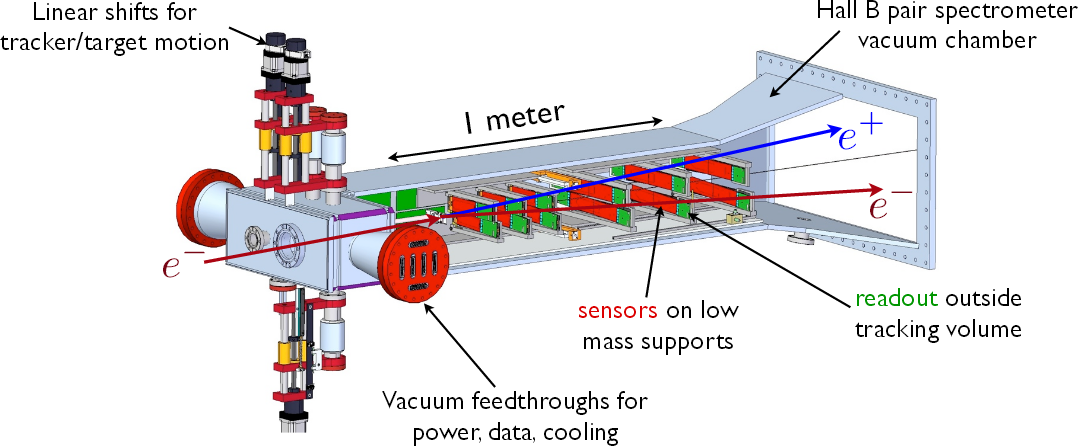
\includegraphics[width=\textwidth]{detector/figs/svt_cutaway}
    \caption{Schematic of the SVT and its support systems.}
    \label{figure:svt_layout}
\end{figure}

\begin{figure}[ht]
    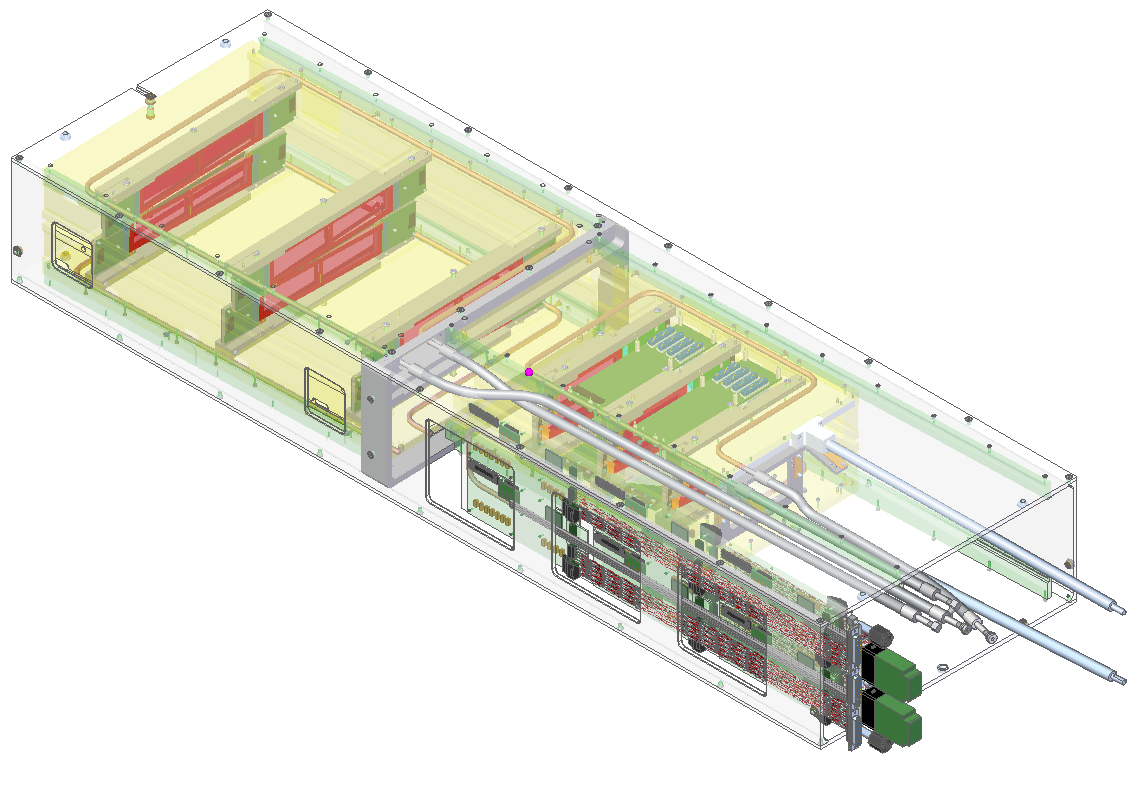
\includegraphics[width=\textwidth]{detector/figs/svt_drawing}
    \caption{Rendering of the SVT as built, showing cooling lines and motion levers.}
    \label{figure:svt_layout}
\end{figure}

\begin{figure}[ht]
    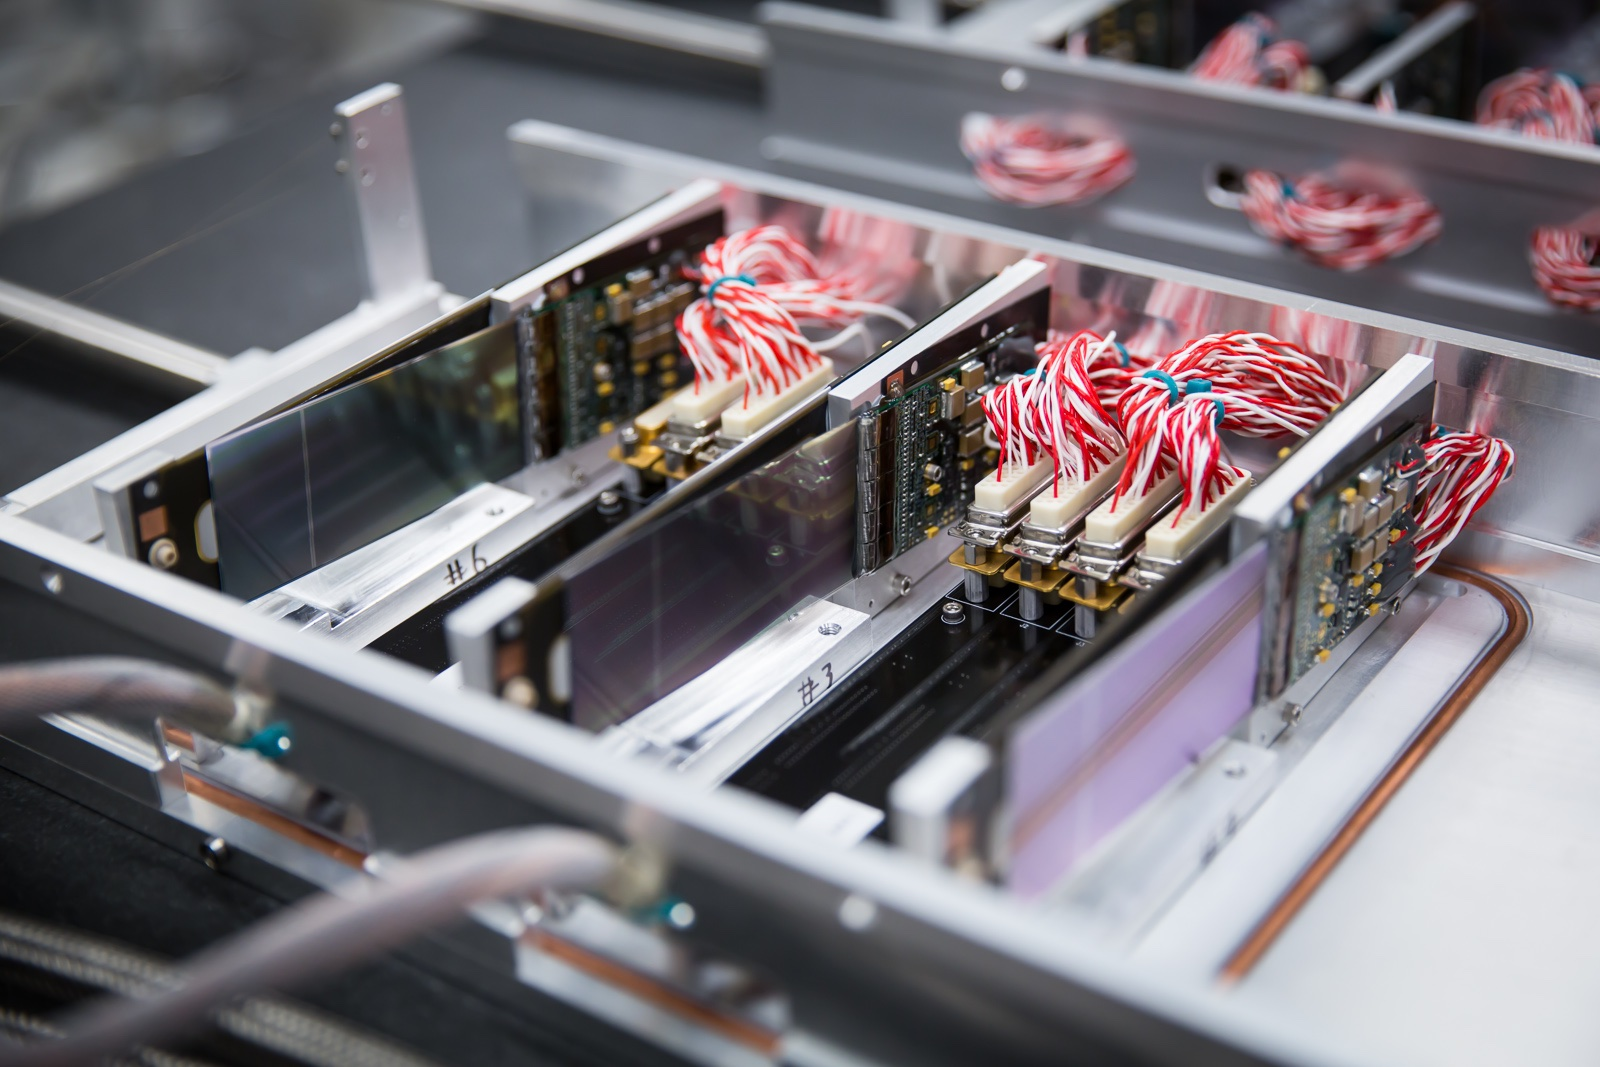
\includegraphics[width=\textwidth]{detector/figs/l123}
    \caption{One of two U-channels for L1-3, fully assembled.}
    \label{figure:svt_layout}
\end{figure}

\begin{figure}[ht]
    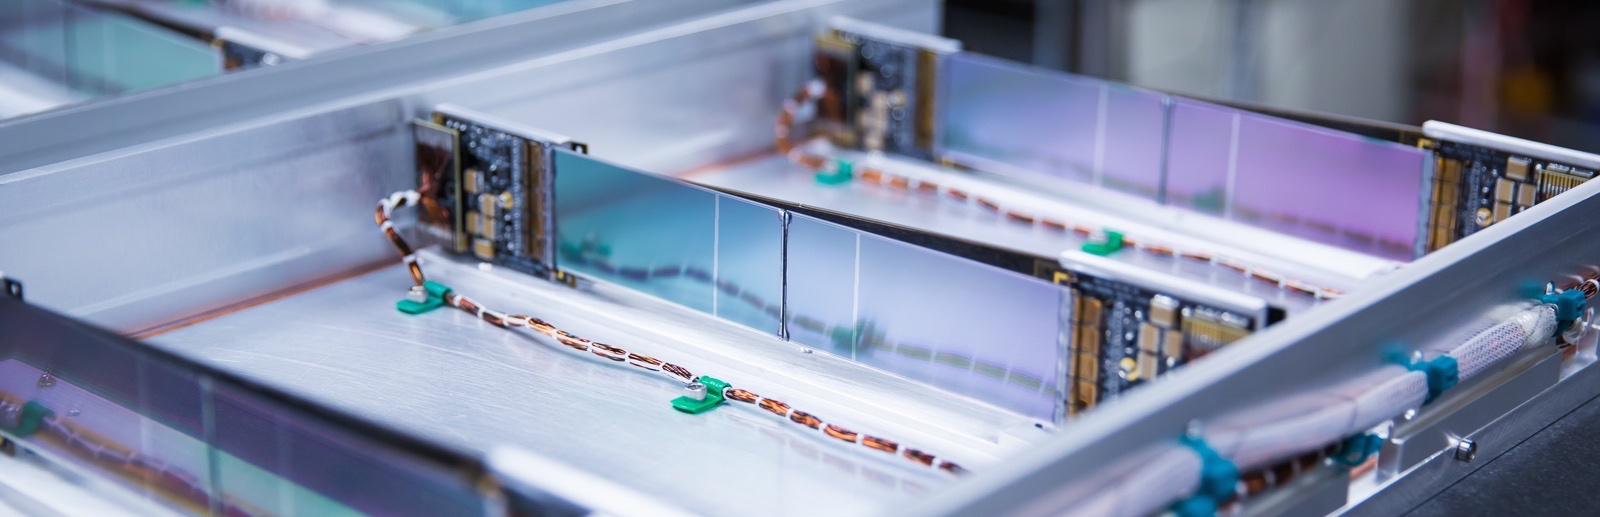
\includegraphics[width=\textwidth]{detector/figs/l456}
    \caption{One of two U-channels for L4-6, fully assembled.}
    \label{figure:svt_layout}
\end{figure}

\begin{figure}[ht]
    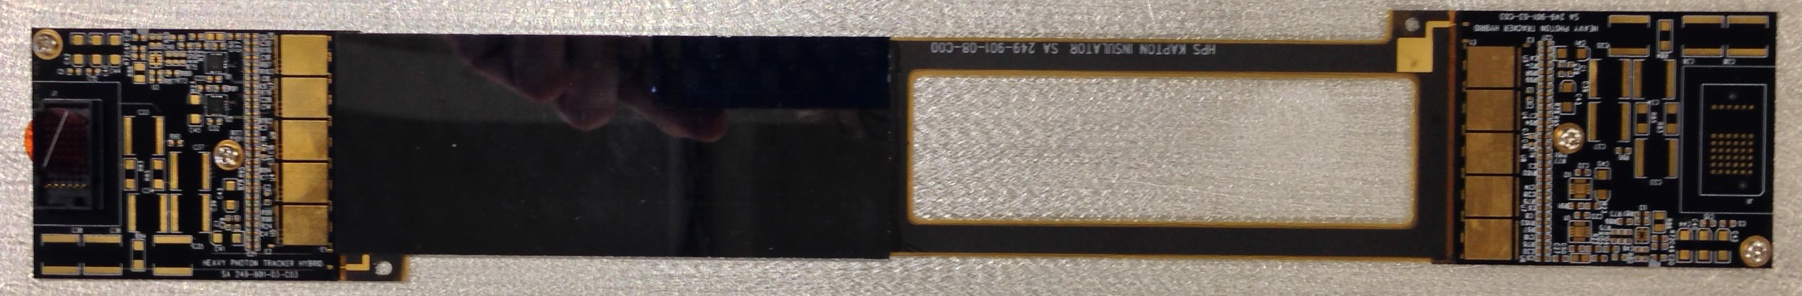
\includegraphics[width=\textwidth]{detector/figs/l456_hm}
    \caption{One half-module for L4-6. The two hybrids (without readout chips, which would be mounted on the gold pads) are at the left and right ends. One sensor is in place, on the left. The carbon fiber support and Kapton passivation layer are visible on the right.}
    \label{figure:svt_layout}
\end{figure}

\begin{figure}[ht]
    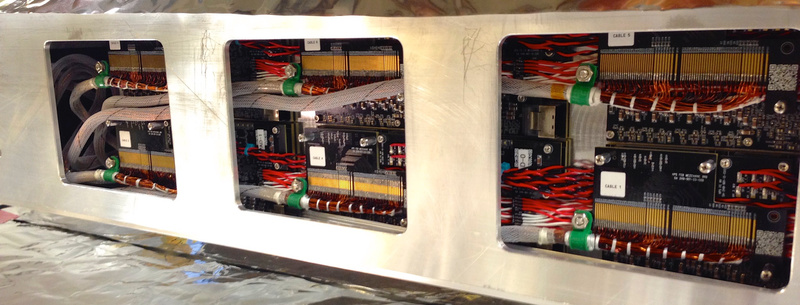
\includegraphics[width=\textwidth]{detector/figs/svt_febs}
    \caption{The SVT FEBs (frontend boards), installed in the SVT box.}
    \label{figure:svt_layout}
\end{figure}

\begin{figure}[ht]
    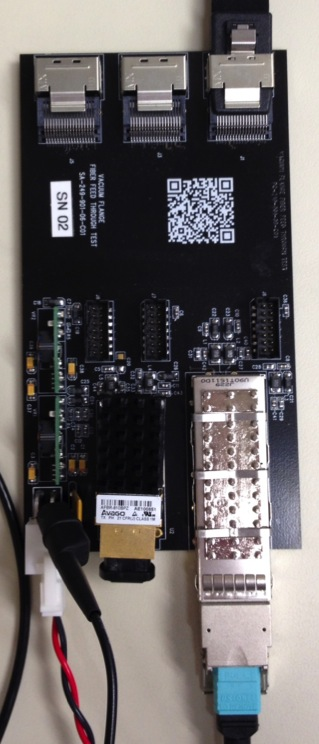
\includegraphics[angle=90,width=\textwidth]{detector/figs/flangeboard}
    \caption{One HPS flange board. The left side of the board operates in vacuum, and has three electrical connectors for high-speed data cables, which connect to the FEBs. The right side of the board operates in air, and has two multi-fiber connectors for data and control signals.}
    \label{figure:svt_layout}
\end{figure}

\begin{figure}[ht]
    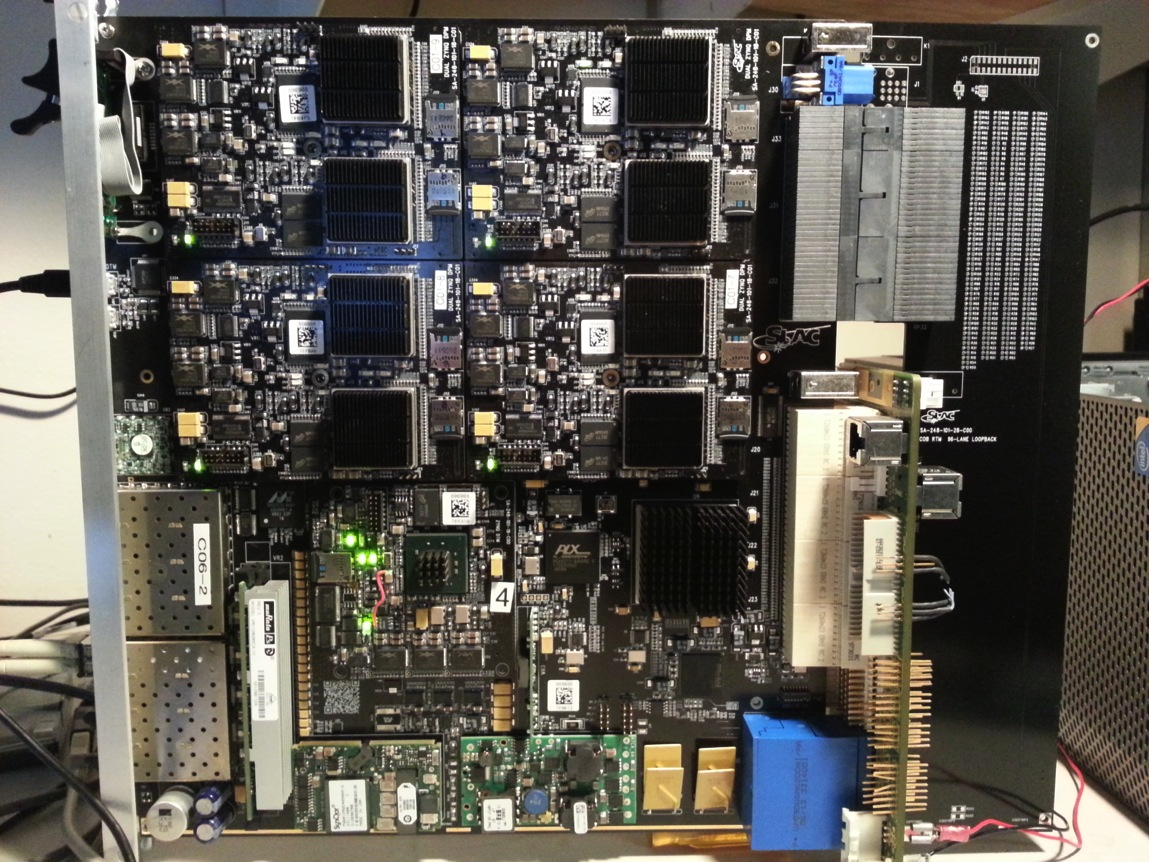
\includegraphics[width=\textwidth]{detector/figs/rce}
    \caption{The RCE system. The COB (Cluster On Board) on the left hosts four RCE (Reconfigurable Cluster Element) daughterboards, which perform the data processing. The RTM (Rear Transition Module) on the right interfaces with fibers carrying data from the flange boards. The COB and RTM would normally be slotted in an ATCA chassis.}
    \label{figure:svt_layout}
\end{figure}


\section{Electromagnetic Calorimeter}
\begin{figure}[ht]
    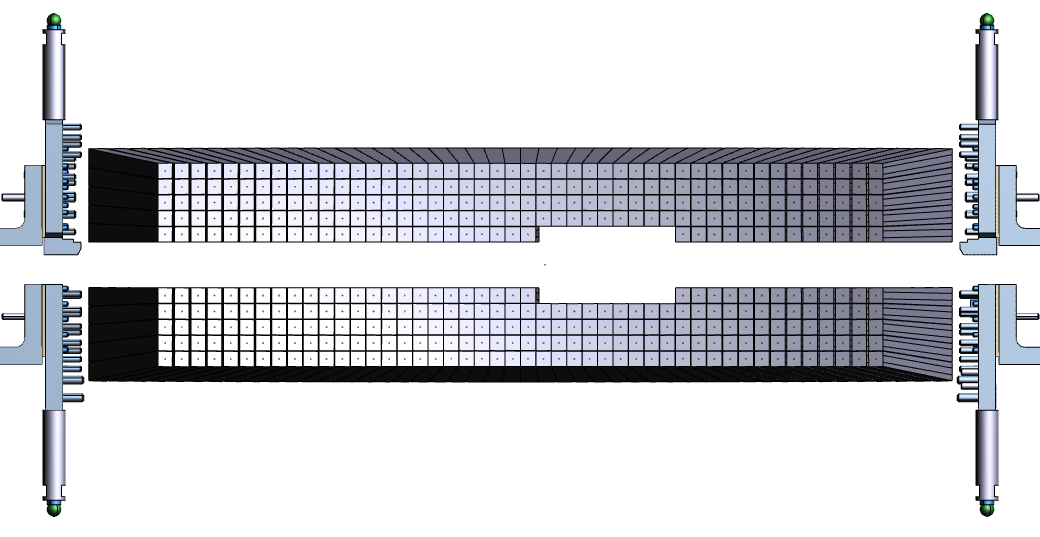
\includegraphics[width=\textwidth]{detector/figs/ECal}
    \caption{Beam's-eye-view of the ECal.}
    \label{figure:svt_layout}
\end{figure}

\begin{figure}[ht]
    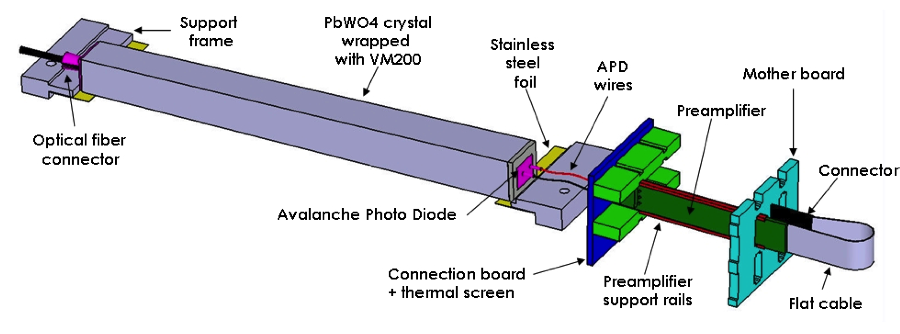
\includegraphics[width=\textwidth]{detector/figs/ecal_module}
    \caption{One ECal crystal with its readout electronics. The optical fiber was used in the CLAS IC for calibration and monitoring, but was removed for HPS. HPS uses LEDs mounted directly in front of the crystals.}
    \label{figure:svt_layout}
\end{figure}

